\section{PDE Discretization}
Multidimensional topological optimization problems often involve the use of partial differential equations (PDEs) which model the physical properties of the materials involved. Most of these PDEs cannot be uniquely solved analytically, so we turn to numerical methods in order to approximate their solutions. The first step in many of these methods is to discretize our domain; that is, we want to choose some scheme to divide our continuous domain into a finite number of pieces over which we will apply a particular method to approximate solutions to the PDE.

The implementation of the SIMP method introduced in $\S$\ref{sec:SIMP} uses the Finite Volume Method to discretize and approximate solutions to the heat equation for the heat generating medium. We will introduce the Heat Equation and then proceed to give an overview of the Finite Volume Method.
\subsection{The Heat Equation}
Consider heat flow through a stationary, inhomogeneous object. The temperature at any point in the interior of the object will depend on the spatial position chosen as well as the time we measure the temperature at that point. Therefore, the temperature ($T$) at any point in such an object is a function of both space ($\mathbf{x}$) and time ($t$) coordinates: $T(\mathbf{x},t)$.
Physical principles require that such a temperature function must satisfy the equation
\begin{equation}
	\frac{\partial T}{\partial t}=\nabla\cdot\left(k(\mathbf{x})\nabla T\right)\label{eqn:HeatEq},
\end{equation}
where $\nabla$ is the gradient operator and the function $k$ represents the thermal diffusivity at a point in our object.

Equation \eqref{eqn:HeatEq} is commonly referred to as the Heat or Diffusion Equation. If we were to have a constant thermal diffusivity throughout our object on a simple domain (such as a square or circle), it would be possible to analytically find a solution to this partial differential equation. However, as in the VP heat conduction problem, when $k$ is not constant we must turn to numerical methods to find approximate solutions for the function $T$.

\begin{figure}
	\centering
	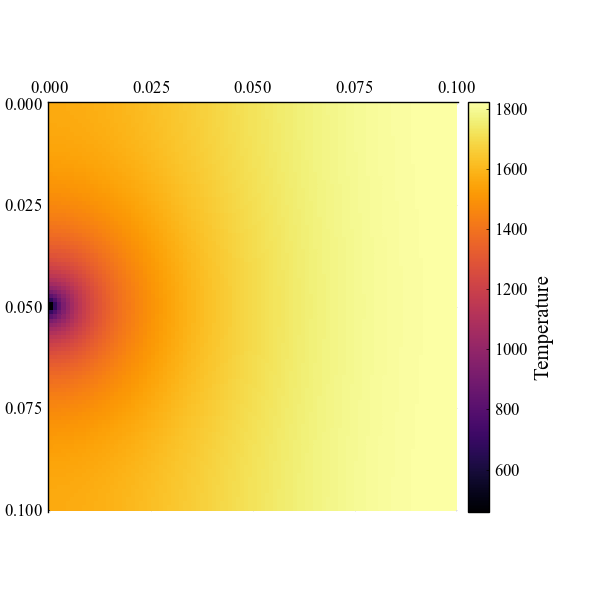
\includegraphics[width=0.8\textwidth]{Chapter_I_Background/Images/Heatmap_Example.png}
	\caption[Heatmap Example]{Heatmap for a \SI{0.1}{\meter} $\times$ \SI{0.1}{\meter} object with uniform heat generation and a heat-sink at the center of its west boundary. This map was produced via the Finite Volume Method using $100\times 100$ uniform control volumes.}
	\label{fig:heatmap-example}
\end{figure}

\subsection{The Finite Volume Method}\label{sec:FVM}

For the numerical approximations of PDEs in this paper the Finite Volume Method (FVM) was implemented, which will be described in this section.

As with many other numerical method to solve PDEs, we must first discretize our domain by creating a mesh. One major advantage of the finite volume method is that it allows for a great amount of freedom in mesh choice. When using FVM the domain can be discretized into a mesh of arbitrary polygons, but uniform squares or rectangles were chosen in our work to simplify the resulting calculations.

Given a mesh of polygons on a domain $\Omega$ with sample points at $\lbrace x_i\rbrace\subset\Omega$, we create a set of \textit{control volumes} around each $x_i$. The resulting set of control volumes will be used to discretize the partial differential equation. The finite volume method has us integrate our PDE over each control volume and then use the Divergence Theorem (\sref{Theorem}{thm:div-thm}) to convert volume integrals into surface integrals involving the fluxes across the boundaries of the control volumes. We then approximate those fluxes across the boundaries to calculate approximate solutions to the PDE of interest, such as \eqref{eqn:HeatEq}.

\begin{thm}[The Divergence Theorem]
	Suppose that $\mathcal{V}$ is a compact subset of $\mathbb{R}^n$ that has a piecewise smooth boundary $\mathcal{S}$ (i.e. $\partial\mathcal{V}=\mathcal{S}$) with outward pointing normal vectors. If $\mathbf{F}$ is a continously differentiable vector field defined on a neighborhood of $\mathcal{V}$, then
	\begin{equation}
		\iiint_{\mathcal{V}}\left(\nabla\cdot\mathbf{F}\right)\dif\mathcal{V}=\oiint_{\mathcal{S}}\left(\mathbf{F}\cdot\mathbf{\hat{n}}\right)\dif\mathcal{S}\label{eqn:div-thm}
	\end{equation}
	where $\hat{\mathbf{n}}$ is the outwards pointing normal vector to the boundary.
	\label{thm:div-thm}
\end{thm}

The divergence theorem is the key component in the finite volume method because it allows us to look at fluxes across the boundaries of each control volume, rather than the control volume itself.

Let us look at the finite volume method applied to the heat equation in two dimensions. Suppose we have discretized our space by dividing it up into a mesh of control volumes $\lbrace V_i\rbrace$. We integrate \eqref{eqn:HeatEq} over each control volume, using the divergence theorem to convert the volume integral into a surface integral:

\begin{equation}
	\int_{V_i}\frac{\partial T}{\partial t}\dif\mathbf{x}=\int_{V_i}\nabla\cdot \left(k(\mathbf{x})\nabla T\right)\dif\mathbf{x}\underset{\eqref{eqn:div-thm}}{=}\int_{\partial V_i}k(\mathbf{x})\nabla T\cdot\hat{\mathbf{n}}\dif s,\label{eqn:Vol-to-Surface-FVM}
\end{equation}

\noindent where $s$ represents the curves that form the boundary of the control volume. Then, applying an approximation scheme to this result, we obtain a sparse and structured linear system. For example, one could apply what is called a ``two-point flux approximation'' scheme which uses finite differences of function values from neighboring cells to the control volume to approximate the flux through the control volume faces \cite{Versteeg2007}.

In a square grid there are only four neighboring cells which we can label as North, South, East, West. For a control volume $V_i$ we'll label the North boundary as $\partial V_N$, the South boundary as $\partial V_S$, the East boundary as $\partial V_E$, and the West boundary as $\partial V_W$. Additionally, let $\Delta x$ be the length of the North and South boundaries, and $\Delta y$ the length of the East and West boundaries. We can discretize \eqref{eqn:Vol-to-Surface-FVM} as
\begin{equation}
	\begin{tabular}{ccc}
		$\displaystyle\int_{\partial V_i}k(\mathbf{x})\nabla T\cdot\hat{\mathbf{n}}\dif s$ & $=$ & $\displaystyle\int_{\partial V_N}k(\mathbf{x})\nabla T\cdot\hat{\mathbf{n}}_N\dif s+\int_{\partial V_S}k(\mathbf{x})\nabla T\cdot\hat{\mathbf{n}}_S\dif s$\\
		 &  & $\displaystyle+\int_{\partial V_E}k(\mathbf{x})\nabla T\cdot\hat{\mathbf{n}}_E\dif s+\int_{\partial V_W}k(\mathbf{x})\nabla T\cdot\hat{\mathbf{n}}_W\dif s$\\
		 & & \\
		 & $\approx$ & $\displaystyle k_N\frac{T_N-T_i}{\|\mathbf{x}_N-\mathbf{x}_i\|}\Delta x+k_S\frac{T_S-T_i}{\|\mathbf{x}_S-\mathbf{x}_i\|}\Delta x$\\
		 & & $\displaystyle+k_E\frac{T_E-T_i}{\|\mathbf{x}_E-\mathbf{x}_i\|}\Delta y+k_W\frac{T_W-T_i}{\|\mathbf{x}_W-\mathbf{x}_i\|}\Delta y$\\
		 & & \\
		 $\displaystyle\implies \Delta x\Delta y\frac{\dif T_i}{\dif t}$ & $=$ & $\displaystyle\left( k_N\frac{T_N-T_i}{\|\mathbf{x}_N-\mathbf{x}_i\|}+k_S\frac{T_S-T_i}{\|\mathbf{x}_S-\mathbf{x}_i\|}\right)\Delta x$\\
		 & & $\displaystyle+\left(k_E\frac{T_E-T_i}{\|\mathbf{x}_E-\mathbf{x}_i\|}+k_W\frac{T_W-T_i}{\|\mathbf{x}_W-\mathbf{x}_i\|}\right)\Delta y$
	\end{tabular}\label{deriv:descrete-FVM}
\end{equation}

The process in \eqref{deriv:descrete-FVM} is repeated for all control volumes $i$ to produce a system of ordinary differential equations which is used to solve for the values of $T_i$.

One other major advantage of the finite volume method is that boundary conditions can easily be taken into account on general domains. For example, adding a heat-sink by applying a Dirichlet boundary condition can be thought of as zeroing out our algebraic equations by introducing a ghost cell that, when interpolated with the boundary cell, causes the temperature across the boundary to be zero.